%%%%%%%%%%%%%%%%%%%%%%%%%%%%%%%%%%%%%%%%%%%%%%%%%%
%% Bachelor's & Master's Thesis Template        %%
%% Copyleft by Dawid Weiss & Marta Szachniuk    %%
%% Faculty of Computing and Telecommunication   %%
%% Poznan University of Technology, 2020        %%
%%%%%%%%%%%%%%%%%%%%%%%%%%%%%%%%%%%%%%%%%%%%%%%%%%


% Szkielet dla pracy licencjackiej pisanej w języku polskim.

\documentclass[english,bachelor,a4paper,oneside]{ppfcmthesis}


\usepackage[utf8]{inputenc}
\usepackage[OT4]{fontenc}
\usepackage{amsmath}
\usepackage{tikz}
\usepackage{subcaption}

%--------------------------------------
% Strona tytułowa
%--------------------------------------

% Autorzy pracy, jeśli jest ich więcej niż jeden
% wstaw między nimi separator \and
\author{%
   Maciej Iwaszkiewicz \album{148275} \and 
   Kamil Kałużny \album{148121} \and
   Jan Krenz \album{148144} \and 
   Piotr Wojsznis \album{147414} } 
\authortitle{}                                % Do not change.

\title{A machine learning system for short-term weather prediction}

% Your supervisor comes here.
\ppsupervisor{prof. PP ~dr hab.~inż.~Wojciech Kotłowski} 

% Year of final submission (not graduation!)
\ppyear{2024}                                 


\begin{document}

% Front matter starts here
\frontmatter\pagestyle{empty}%
\maketitle\cleardoublepage%


%--------------------------------------
% Spis treści
%--------------------------------------

\pagenumbering{Roman}\pagestyle{ppfcmthesis}%
\tableofcontents* 
\cleardoublepage % Zaczynamy od nieparzystej strony

%--------------------------------------
% Rozdziały
%--------------------------------------

%Najwygodniej jeśli każdy rozdział znajduje się w oddzielnym pliku
\mainmatter%

\chapter{Introduction}

\section{Abstract}
The drastically changing climate in recent times has led to a significant increase in interest in the research related to modeling weather and meteorological phenomena. Machine learning scientists are trying to surpass the previous state-of-the-art methods in this field, that leverage numerical computations. 

Given that weather states can be interpreted as highly complex dynamical systems, utilizing deep learning methods appears reasonable due to their flexibility and proficiency in handling complex data. These attributes make them a potentially successful group of techniques in this field.

Attributable to the above statements, in our work, we want to present the forecasting capabilities of straightforward methods of classical machine learning as well as design a more complex model based on graph neural networks. In addition, we will compare the quality of distinct solutions and create a full system with a mobile application presenting the predictive skills of the created architecture. Finally, in a notable achievement, we will integrate our top-performing solution with an arbitrarily selected approach from the numerical weather prediction paradigm -- improving its predictive performance. This accomplishment underscores the potential of enhancing numerical methods through integrating them with advanced deep-learning solutions.

\section{Motivation}
At the present rate of progress, machine learning methods are applied and often give great promise in almost all areas of our lives. With this work, we would like to add our contribution to this issue with regard to the problem of short-term weather prediction. Until now, the models obtaining the finest results in this area belong to the "Numerical Weather Prediction" (NWP) family. An example of such a solution might be IFS \cite{ECMWFIFS}, incorporated by EMCWF -- "European Centre for Medium-Range Weather Forecasts". Their most significant weakness is that they are computationally very expensive. Supercomputers generating serious carbon footprints are often needed for the model to run effectively. These models attempt to solve complex differential equations with very high precision. Moreover, their prediction time is often very long. 
For this reason, machine learning-based solutions from the "Machine Learning Weather Prediction" (MLWP) family are becoming increasingly popular, therefore we want to focus on them in our work. The particular example that caused us to get interested in the topic was the publication of a paper "Learning skillful medium-range global weather forecasting" \cite{lam2023graphcast} about GraphCast, further described in Section \ref{sec:graphcast}. 

(pros cons of both NWP, MLWP?)

\section{Goals}
One of the main goals is to implement and compare the performance of various machine learning models for examined task. Additionally, we want to obtain sufficient results that allow us to support the thesis that graph neural networks and generally machine learning approaches for weather prediction tasks are promising and worth developing.

\section{Scope}
\subsection{Dataset}
During our work, we have used the Copernicus Climate Change Service (C3S) Climate Data Store (CDS) "ERA5 hourly data on single levels from 1940 to present" dataset \cite{ERA5}. It contains regularly updated hourly global weather data from 1940 to present -- usually with about 5 days of latency. It is provided by the European Centre for Medium-Range Weather Forecasts (EMCWF) and combines vast amounts of historical observations into global estimates using advanced modelling and data assimilation systems. There are many atmospheric, ocean-wave and land-surface quantities inside, however we have decided to focus on 6 features (Table \ref{tab:data_features}).

\begin{table}[!ht]
\centering
\begin{tabular}{|c|c|c|}
     \hline
     Symbol & Quantity & Unit \\
     \hline
     t2m & Temperature at 2m above ground & $^{\circ}$C \\
     sp & Surface pressure & hPa \\
     tcc & Total cloud cover & (0 - 1) \\
     u10 & 10m U wind component & $m/s$ \\
     v10 & 10m V wind component & $m/s$ \\
     tp & Total precipitation & mm \\
     \hline
     lsm & Land-sea mask (not predicted) & (0 - 1) \\
     z & Geopotential (not predicted) & $m^2/s^2$ \\
     \hline
\end{tabular}
\caption{Weather features we considered. Some of the units differ from those provided in the dataset. These have been converted for our convenience}
\label{tab:data_features}
\end{table}

These features were determined by us to be the most useful, and during our proceedings the models will attempt to accurately predict them. Apart from the self-explanatory, the U and V wind components represent the speed of wind moving towards the east and the north respectively. We also used 2 other quantities that provide additional information to our neural network models -- a binary land-sea mask and geopotential, which is the gravitational potential energy of a unit mass, which can be interpreted as a measure of orography. These two features are never predicted.

During our work, we have used many different timespans of the dataset, always from 2018 - 2023. Most commonly, we used 2019 - 2022, since that can be easily divided into the training, validation, and test datasets, with each having a full year worth of data. More details on our use of the dataset can be found in Section \ref{chap:dataset}.

\subsection{Models}
The research part of our thesis will be primarily devoted to the implementation and analysis of machine learning models. Based on the literature review, we will attempt to leverage the techniques used in examined state-of-the-art solutions into our primary model. For all implemented solutions, we will conduct numerous experiments checking, among other things, the quality of forecasting depending on the length of the model's input sequence (i.e., the past time steps the model has access to) and also how the models perform with increasing forecasting horizon (the number of forecasted future time steps). In addition, to obtain the estimation of optimal performance per model, we will perform hyperparameter optimizations for each. Lastly, we will compare the quality of prediction with the ERA5 dataset adopted as ground truth weather states and the topline solution, based on the Numerical Weather Prediction paradigm. 
% Survey multiple machine learning models and a lighter version of GraphCast architecture. Perform experiments, compare results with ground truth weather states dataset ERA5 and SOTA/topline solution based on fluid dynamics or other related to Numerical Weather Prediction approach.

\subsection{App}
In this section of the thesis, we will focus on another aspect of our machine learning system for short-term weather prediction – the mobile application and its integration with an API. Our primary goal is to examine the functionality and structure of the application, serving as a conduit for users to access predictions generated by our model.

The application plays a pivotal role in facilitating communication with our machine learning model through an Application Programming Interface (API). This enables users to access predictive insights seamlessly, providing an accessible means to leverage advanced weather forecasting. Utilizing Android Studio, Google's official integrated development environment for Android, the mobile application is designed to offer a user-friendly experience. The emphasis is not only on the predictions but also on ensuring the application's overall functionality and structure allow users to navigate and interpret information effortlessly.

Additionally, we explore the architecture of the API supporting this system. As a critical component in enabling communication between the application and the machine learning model, we delve into the construction and deployment of the API, essential for the robustness and reliability of our system.


\section{Methodology}
The most crucial foundation of any project developed within a group is effective communication and planning of undertaken actions. Central to our approach is the adoption of Agile principles, emphasizing adaptability and collaboration throughout the project's lifecycle.

Agile methodology served as the guiding framework, allowing us to navigate the complexities of software development. A pivotal aspect of our methodology involves weekly, digital live-coding sessions. These sessions foster real-time collaboration among team members, enabling them to collectively address challenges, share insights, and iteratively refine the codebase. They also served as a good motivation to consistently start working, knowing that there would always be someone to help overcome any obstacles encountered. The fluidity of live-coding sessions aligns with Agile principles, ensuring that our development process remains responsive to evolving requirements and feedback.

In addition to live-coding, our methodology incorporates brainstorming sessions as a means to cultivate creative problem-solving and ideation. These collaborative gatherings serve as a forum for team members to share perspectives, propose innovative solutions, and collectively shape the trajectory of the project. By fostering an environment conducive to open dialogue and idea exchange, we harness the collective intelligence of the team to make informed decisions and enhance the overall quality of our machine learning system.

Furthermore, we employed modern collaborative tools to streamline our development process. Code is stored and shared through GitHub, providing a centralized repository for version control and collaborative code management. Communication within the team was facilitated through platforms such as Discord and Messenger, enabling real-time discussions, progress updates, and quick resolution of queries. These tools played a pivotal role in enhancing communication and coordination, essential elements in the successful execution of an Agile methodology within a team setting.

These methods contributed to the flexibility and responsiveness crucial for successfully navigating the challenges inherent in the development of a complex machine learning system. 

\section{Author-Specific Contributions}
\chapter{Theoretical introduction}
	
\section{Problem introduction}
 Theoretical introduction to a problem and mathematical concepts, literature review.... \\
 
\noindent General task is to predict a weather state $\Omega_t$, observed at a timestamp $t$, given $s$ steps from the past, which are essentially previous weather states: $(\Omega_{t-1}, ..., \Omega_{t-s})$. We define $\Omega_t$ as a tensor of a shape: (latitude span, longitude span, features), therefore our complete input data would be 4-dimensional with additional dimension for a time \footnote{To be precise, for neural network based solutions it will be 5-dimensional due to the usage of batches.}. Spatial span was selected so as to cover the border of the whole of Poland and some of its neighbors. More details regarding data are discussed in dataset chapter~\ref{chap:dataset}. High-level spatio-temporal prediction framework is presented at Figure ~\ref{fig:in_out}. \\


\newpage
\subsection{Naming conventions and general prediction framework}
 For further convenience, we propose a general naming convention. 
 \begin{table}[!h]
    \centering
     \begin{tabular}{|c|c|}
        \hline
        Symbol & Description \\
        \hline
        $f_i$ & i-th feature \\
        $s$ & Number of past steps \\
        $fh$ & Forecasting horizon \\
        $\Omega$ & Weather state for all features \\
        $\mathbf{X}$ & $s$-element set of $\Omega$  \\
        $X_t$ & $\Omega$ for timestamp t\\
        $\mathbf{\hat{Y}}$ & $fh$-element set of estimated $\Omega$ \\
        $\hat{Y_t}$ & Estimate of $\Omega$ for timestamp t \\
        $\hat{y_t}^{f_j}$ & Estimate of $\Omega$ for timestamp t and feature $f_j$ \\
        \hline
    \end{tabular}
    \caption{General conventions}
 \end{table}
 
 
%% \noindent We define a $\mathbf{\Phi}$ as a set of baseline models that consist of: 
\begin{table}[!h]
    \centering
    \begin{tabular}{|c|c|}
        \hline
        Model Notation & Model Description \\
        \hline
        $\mathbf{\Phi}_{slr}$ & Simple Linear Regression \\
        $\mathbf{\Phi}_{lr}$  & Linear Regression \\
        $\mathbf{\Phi}_{es}$  & Exponential Smoothing \\
        $\mathbf{\Phi}_{gb}$ & Gradient Boosting Trees \\
        \hline
    \end{tabular}
\caption{Model conventions}
\end{table}
 
%% \noindent Additionally, due to the fact that model $\mathbf{\Phi}_i$ consist of independent models that predicts single feature $f_j$ of a weather state, we can divide it into: 
 
 \noindent Additionally, we define a model $\mathbf{\Phi}_i$ as a set of independent sub-models, where each is responsible only for the prediction of feature $f_j$. This solution was proposed to avoid situations in which ... TODO.
 \[
 \mathbf{\Phi}_{i} = (\Phi_{i}^{f_1}, ..., \Phi_{i}^{f_n})
 \]
 In further considerations, we will use a term sub-models for each of $\Phi_{i}^{f_j}$.


\begin{figure}[!h]

\tikzset{every picture/.style={line width=0.75pt}} %set default line width to 0.75pt        

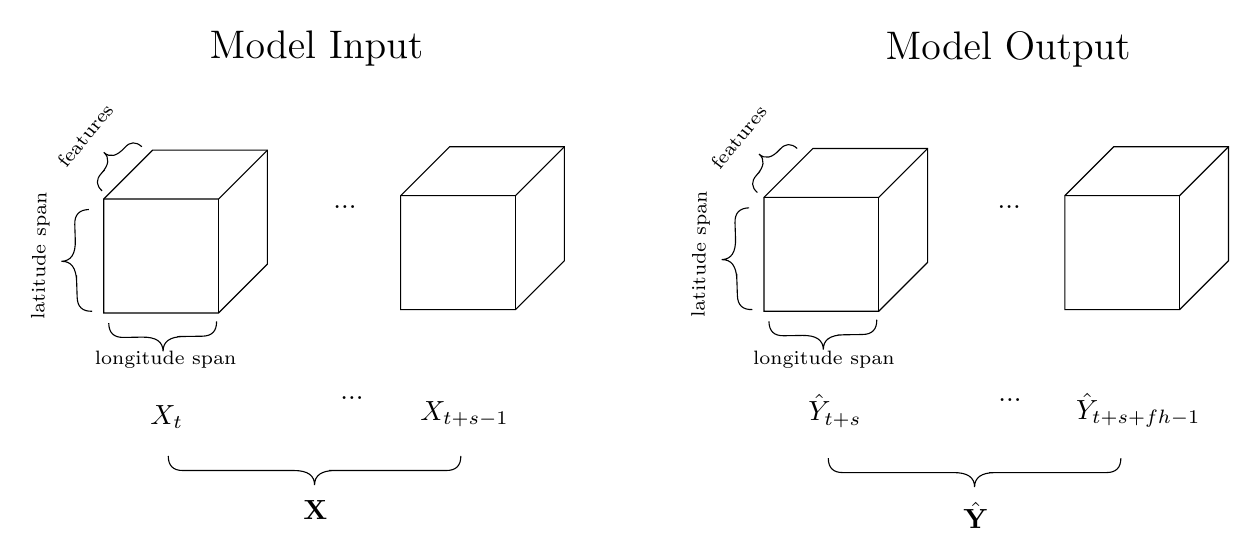
\begin{tikzpicture}[x=0.75pt,y=0.75pt,yscale=-1,xscale=1]
%uncomment if require: \path (0,389); %set diagram left start at 0, and has height of 389

%Shape: Cube [id:dp2816308175879604] 
\draw   (58.25,114.54) -- (81.78,91.01) -- (137.08,91.01) -- (137.08,145.91) -- (113.55,169.44) -- (58.25,169.44) -- cycle ; \draw   (137.08,91.01) -- (113.55,114.54) -- (58.25,114.54) ; \draw   (113.55,114.54) -- (113.55,169.44) ;
%Shape: Brace [id:dp4309828249836092] 
\draw   (76.63,89.37) .. controls (73.72,86.74) and (70.94,86.88) .. (68.31,89.8) -- (68.31,89.8) .. controls (64.55,93.97) and (61.21,94.73) .. (58.29,92.1) .. controls (61.21,94.73) and (60.79,98.13) .. (57.03,102.29)(58.72,100.42) -- (57.03,102.29) .. controls (54.4,105.21) and (54.54,107.99) .. (57.45,110.62) ;
%Shape: Brace [id:dp7756675475750493] 
\draw   (51.06,119.6) .. controls (46.39,119.75) and (44.14,122.16) .. (44.29,126.83) -- (44.53,134.35) .. controls (44.75,141.01) and (42.53,144.42) .. (37.86,144.57) .. controls (42.53,144.42) and (44.97,147.67) .. (45.19,154.34)(45.09,151.34) -- (45.43,161.86) .. controls (45.58,166.52) and (47.99,168.77) .. (52.66,168.62) ;
%Shape: Brace [id:dp612063156099937] 
\draw   (60.65,174.34) .. controls (60.72,179.01) and (63.09,181.3) .. (67.76,181.23) -- (76.73,181.09) .. controls (83.4,180.98) and (86.77,183.26) .. (86.84,187.93) .. controls (86.77,183.26) and (90.06,180.88) .. (96.73,180.78)(93.73,180.82) -- (105.71,180.64) .. controls (110.38,180.57) and (112.67,178.2) .. (112.6,173.53) ;
%Shape: Cube [id:dp42835259632452516] 
\draw   (201.31,112.9) -- (224.84,89.37) -- (280.14,89.37) -- (280.14,144.28) -- (256.61,167.81) -- (201.31,167.81) -- cycle ; \draw   (280.14,89.37) -- (256.61,112.9) -- (201.31,112.9) ; \draw   (256.61,112.9) -- (256.61,167.81) ;
%Shape: Brace [id:dp07592439753840141] 
\draw   (89.33,238.35) .. controls (89.33,243.02) and (91.66,245.35) .. (96.33,245.35) -- (149.81,245.35) .. controls (156.48,245.35) and (159.81,247.68) .. (159.81,252.35) .. controls (159.81,247.68) and (163.14,245.35) .. (169.81,245.35)(166.81,245.35) -- (223.29,245.35) .. controls (227.96,245.35) and (230.29,243.02) .. (230.29,238.35) ;
%Shape: Cube [id:dp7110500253196546] 
\draw   (376.35,113.72) -- (399.88,90.19) -- (455.18,90.19) -- (455.18,145.09) -- (431.65,168.62) -- (376.35,168.62) -- cycle ; \draw   (455.18,90.19) -- (431.65,113.72) -- (376.35,113.72) ; \draw   (431.65,113.72) -- (431.65,168.62) ;
%Shape: Brace [id:dp86120893233015] 
\draw   (392.33,90.19) .. controls (389.42,87.56) and (386.64,87.7) .. (384.01,90.62) -- (384.01,90.62) .. controls (380.25,94.78) and (376.91,95.54) .. (373.99,92.91) .. controls (376.91,95.54) and (376.49,98.94) .. (372.73,103.11)(374.42,101.24) -- (372.73,103.11) .. controls (370.1,106.02) and (370.24,108.8) .. (373.15,111.43) ;
%Shape: Brace [id:dp9673653209625941] 
\draw   (369.15,118.79) .. controls (364.49,118.94) and (362.24,121.34) .. (362.39,126.01) -- (362.63,133.53) .. controls (362.85,140.2) and (360.63,143.6) .. (355.96,143.75) .. controls (360.63,143.6) and (363.07,146.86) .. (363.28,153.52)(363.19,150.52) -- (363.53,161.04) .. controls (363.68,165.71) and (366.09,167.96) .. (370.75,167.81) ;
%Shape: Brace [id:dp9113296386668477] 
\draw   (378.74,173.53) .. controls (378.81,178.2) and (381.18,180.49) .. (385.85,180.42) -- (394.83,180.27) .. controls (401.5,180.17) and (404.87,182.45) .. (404.94,187.12) .. controls (404.87,182.45) and (408.16,180.07) .. (414.83,179.96)(411.83,180.01) -- (423.8,179.82) .. controls (428.47,179.75) and (430.76,177.38) .. (430.69,172.71) ;
%Shape: Cube [id:dp35039842919754816] 
\draw   (521.31,112.9) -- (544.84,89.37) -- (600.14,89.37) -- (600.14,144.28) -- (576.61,167.81) -- (521.31,167.81) -- cycle ; \draw   (600.14,89.37) -- (576.61,112.9) -- (521.31,112.9) ; \draw   (576.61,112.9) -- (576.61,167.81) ;
%Shape: Brace [id:dp3763157845274283] 
\draw   (407.33,239.35) .. controls (407.33,244.02) and (409.66,246.35) .. (414.33,246.35) -- (467.81,246.35) .. controls (474.48,246.35) and (477.81,248.68) .. (477.81,253.35) .. controls (477.81,248.68) and (481.14,246.35) .. (487.81,246.35)(484.81,246.35) -- (541.29,246.35) .. controls (545.96,246.35) and (548.29,244.02) .. (548.29,239.35) ;

% Text Node
\draw (33.24,96.31) node [anchor=north west][inner sep=0.75pt]  [rotate=-309.39,xslant=-0.03] [align=left] {{\scriptsize features}};
% Text Node
\draw (79.43,212.59) node [anchor=north west][inner sep=0.75pt]    {$X_{t}$};
% Text Node
\draw (167.65,116.51) node [anchor=north west][inner sep=0.75pt]   [align=left] {...};
% Text Node
\draw (21.86,173.65) node [anchor=north west][inner sep=0.75pt]  [rotate=-270.99] [align=left] {{\scriptsize latitude span}};
% Text Node
\draw (52.73,186.5) node [anchor=north west][inner sep=0.75pt]   [align=left] {{\scriptsize longitude span}};
% Text Node
\draw (209.49,210.96) node [anchor=north west][inner sep=0.75pt]    {$X_{t+s-1}$};
% Text Node
\draw (171.04,208.29) node [anchor=north west][inner sep=0.75pt]   [align=left] {...};
% Text Node
\draw (153.16,258.53) node [anchor=north west][inner sep=0.75pt]    {$\mathbf{X}$};
% Text Node
\draw (433.72,32.89) node [anchor=north west][inner sep=0.75pt]   [align=left] {{\Large Model Output}};
% Text Node
\draw (108.05,32.26) node [anchor=north west][inner sep=0.75pt]   [align=left] {{\Large Model Input}};
% Text Node
\draw (348.14,97.12) node [anchor=north west][inner sep=0.75pt]  [rotate=-309.39,xslant=-0.03] [align=left] {{\scriptsize features}};
% Text Node
\draw (339.95,172.84) node [anchor=north west][inner sep=0.75pt]  [rotate=-270.99] [align=left] {{\scriptsize latitude span}};
% Text Node
\draw (369.83,186.68) node [anchor=north west][inner sep=0.75pt]   [align=left] {{\scriptsize longitude span}};
% Text Node
\draw (487.65,116.51) node [anchor=north west][inner sep=0.75pt]   [align=left] {...};
% Text Node
\draw (396.43,207.59) node [anchor=north west][inner sep=0.75pt]    {$\hat{Y}_{t+s}$};
% Text Node
\draw (525.49,206.96) node [anchor=north west][inner sep=0.75pt]    {$\hat{Y}_{t+s+fh-1}$};
% Text Node
\draw (488.04,209.29) node [anchor=north west][inner sep=0.75pt]   [align=left] {...};
% Text Node
\draw (471.16,259.53) node [anchor=north west][inner sep=0.75pt]    {$\hat{\mathbf{Y}}$};


\end{tikzpicture}


\label{fig:in_out} \caption{Spatio-Temporal prediction framework} 

\end{figure}


\noindent Take into account the fact that this framework may differ when applying techniques such as grid neighbors~\ref{chap:neighbors} or using constants encodings~\ref{chap:feat_eng}. Details regarding those differences are explained deeply in subsequent chapters.

 \newpage
 
 \subsection{Literature review}
 After stating the problem we want to shortly inspect current research and results in this field... \\
Short review of quality papers related to this problem; explanation of what was already achieved in this task - SOTA solutions, especially emphasizing GraphCast paper; what we want to reproduce or compare ourself with. \\
\noindent Maybe start with: ~\cite{WFConsiderations}

\section{Explored techniques}
 \subsection{Autoregression}
 \noindent Each baseline model is designed to predict the entire weather state for only the next timestamp - unit forecasting horizon. Therefore, when applying our models for short-term prediction task of a few timestamps into the future, the autoregressive approach is commonsensical. \\ \\
 
 \noindent Let's define model input as $\mathbf{X}$, a vector of $s$ weather states: 
 \[
 \mathbf{X} = (X_{t}, ..., X_{t+s-1})
 \]
 and output of a model as $\mathbf{\hat{Y}}$, which consist of $fh$ forecasted states:
 \[
 \mathbf{\hat{Y}} = (\hat{Y}_{t+s}, ..., \hat{Y}_{t+s+fh-1})
 \]
 
 \noindent Autoregressive prediction is $fh$-steps process such that:
 \begin{flalign*}
    &\hat{Y}_{t+s} = \mathbf{\Phi}_{i}(X_{t}, ..., X_{t+s-1}) \\
    &\hat{Y}_{t+s+1} = \mathbf{\Phi}_{i}(X_{t+1}, ..., X_{t+s-1}, \hat{Y}_{t+s}) \\
    &\vdots \\
    &\hat{Y}_{t+s+fh-1} = \mathbf{\Phi}_{i}(X_{t+fh-1}, ...,  \hat{Y}_{t+s+fh-3}, \hat{Y}_{t+s+fh-2})
 \end{flalign*}

 \noindent Therefore, oversimplifying:
 \[
    \mathbf{\hat{Y}} = \mathbf{\Phi_{i}(X)}
 \]
 
 \noindent For each model except $\mathbf{\Phi}_{slr}$, during every autoregressive step concatenation of outputs from sub-models is required, whereas $X_t$ needs to have information from every feature:
 \begin{flalign*}
    &\hat{y}_t^{f_j} = \Phi_{i}^{f_j}(\mathbf{X}) \\
    &\hat{Y}_{t} = (\hat{y}_t^{f_0}, ..., \hat{y}_t^{f_n}) \\
 \end{flalign*}
 
\newpage
\subsection{Grid Neighbors}\label{chap:neighbors}

\noindent For each input tensor we've implemented though called additional neighbors technique. It is expanding each of our data points to store information about closely located grid boxes. They're chosen based on the relative distance (radius) between the center of grid-boxes: $r$. On underneath figure, grid boxes colored grey represents relative data point and black boxes are its neighbors.

\begin{figure}[!ht]
    \centering
    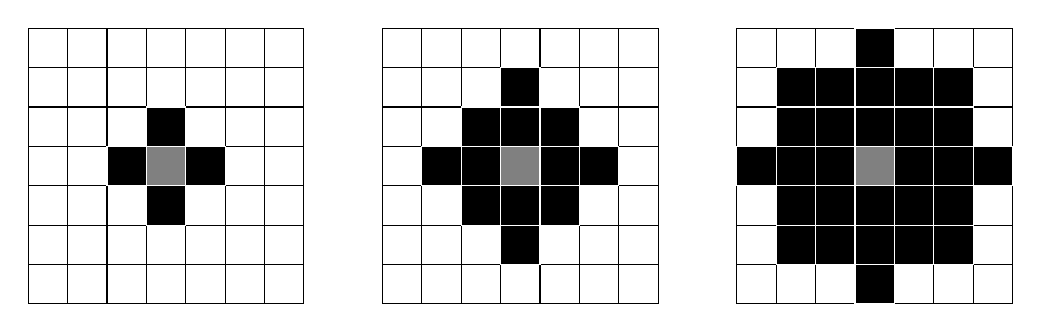
\begin{tikzpicture}[scale=0.5]
        \draw[step=1, black] (0,0) grid (7,7);
        \filldraw[fill=gray, draw=white] (3,3) rectangle (4,4);
        \filldraw[fill=black, draw=white] (3,2) rectangle (4,3);
        \filldraw[fill=black, draw=white] (2,3) rectangle (3,4);
        \filldraw[fill=black, draw=white] (3,4) rectangle (4,5);
        \filldraw[fill=black, draw=white] (4,3) rectangle (5,4);
        
        \begin{scope}[shift={(9,0)}]
            \draw[step=1, black] (0,0) grid (7,7);
            \foreach \i in {1, ..., 9} {
                \pgfmathtruncatemacro\row{mod(\i-1,3)}
                \pgfmathtruncatemacro\col{int((\i-1)/3)}
                \filldraw[fill=black, draw=white] (\row+2,\col+2) rectangle (\row+3,\col+3);
            }
            \filldraw[fill=gray, draw=white] (3,3) rectangle (4,4);
            \filldraw[fill=black, draw=white] (1,3) rectangle (2,4);
            \filldraw[fill=black, draw=white] (5,3) rectangle (6,4);
            \filldraw[fill=black, draw=white] (3,1) rectangle (4,2);
            \filldraw[fill=black, draw=white] (3,5) rectangle (4,6);
        \end{scope}

        \begin{scope}[shift={(18,0)}]
            \draw[step=1, black] (0,0) grid (7,7);
            \foreach \i in {1, ..., 25} {
                \pgfmathtruncatemacro\row{mod(\i-1,5)}
                \pgfmathtruncatemacro\col{int((\i-1)/5)}
                \filldraw[fill=black, draw=white] (\row+1,\col+1) rectangle (\row+2,\col+2);
            }
            \filldraw[fill=gray, draw=white] (3,3) rectangle (4,4); 
            \filldraw[fill=black, draw=white] (0,3) rectangle (1,4);
            \filldraw[fill=black, draw=white] (6,3) rectangle (7,4);
            \filldraw[fill=black, draw=white] (3,0) rectangle (4,1);
            \filldraw[fill=black, draw=white] (3,6) rectangle (4,7);
        \end{scope}
    \end{tikzpicture}
    \caption{Neighbors logic for $r=(1,2,3)$}
    \label{fig:neighbors}
\end{figure}

%Formal definition of a neighbors set $N$ for all of grid boxes $v$, where $V$ is a set of all:
\noindent Formal definition, assuming that grid boxes has resolution (1x1):
\begin{table}[!h]
    \centering
    \begin{tabular}{|c|c|}
        \hline
        Symbol & Description \\
        \hline
        $v_{i,j}$ & Grid box at latitude $i$ and longitude $j$ \\
        $V$  & Set of all grid boxes \\
        $\|v_{m,n} - v_{i,j}\|^2$  & Euclidian distance between centres of $v_1$ and $v_2$ \\
        $N_v$ & Set of neighbors for grid box $v$ \\
        \hline
    \end{tabular}
\end{table}
\[
    \forall v_{i,j} \in V: \{\forall v_{m,n \neq i,j} : \|v_{m,n} - v_{i,j}\|^2 \le r\} \in N_{v_{i,j}}
\]

\noindent Unfortunately, the trade-off between memory footprint, computational complexity, and performance gain was not sufficient to incorporate and test bigger $r$ values.

 
 \section{Baselines}
 \subsection{Exponential Smoothing}
 \subsection{Simple Linear Regression}
 \subsection{Linear Regression}
 
 \[
    \mathbf{X} \boldsymbol\beta = \mathbf{\hat{Y}}
 \]
 
 \[
    \begin{bmatrix}
    x_{11} & x_{12} & \cdots & x_{1n}\\
    x_{21} & x_{22} & \cdots & x_{2n}\\
    \vdots & \vdots & \ddots & \vdots\\
    x_{n1} & x_{n2} & \cdots & x_{nn}
    \end{bmatrix}
    \begin{bmatrix}
    \beta_1\\\beta_2\\ \vdots\\b_n
    \end{bmatrix}
    =\begin{bmatrix}
    \hat{y_1}\\\hat{y_2}\\ \vdots\\\hat{y_n}
    \end{bmatrix}
\]
 \subsection{Gradient Boosting}
 \subsection{UNet}


\section{Neural network concept}
Optional? \\

\noindent Explain architecture of dense neural networks and other types such as convolutional, recurrent, graph (depending on which one eventually will be used).

\section{GraphCast}
Deep dive into GraphCast architecture.

\section{Model}
Proposed model architecture and comparision with GraphCast. \\

\noindent After briefly testing multiple Graph Convolutional Cells that support edge feature vectors, we have concluded that the most promising results and sufficient computation time are obtained by TransformerConv ~\cite{shi2021masked}.\\

\noindent Multi-layer perceptron as an embedder converting features dimension into more abstract latent space that stores better representation of weather state.

.... \\

\noindent Multi-layer perceptron as a decoder converting encoded features into its natural representation.


\begin{flalign*}
    X = MLP^{Embedder}(X) \\
    X = GNN_1(X) \\
    ...         \\
    X = GNN_N(X) \\
    \hat{Y} = MLP^{Decoder}(X) \\
 \end{flalign*}

\subsection{Additional techniques and feature engineering}\label{chap:feat_eng}
Present concept of spatial-mapping, edge attributes. Explain spatial and temporal feature encodings as well as usage of constants like geopotential. 

\begin{flalign*}
    d_{V_i,V_j} &= \sqrt{(V_{j_x} - V_{i_x})^2 + (V_{j_y} - V_{i_y})^2} \\
    e_{V_i,V_j} &= (V_{j_x} - V_{i_x}, V_{j_y} - V_{i_y}, d_{V_i,V_j})
\end{flalign*}
 

\chapter{Report and analysis}\label{chap:report}

\section{Project structure}
\begin{figure}[!ht]
    \tikzset{every picture/.style={line width=0.75pt}} 
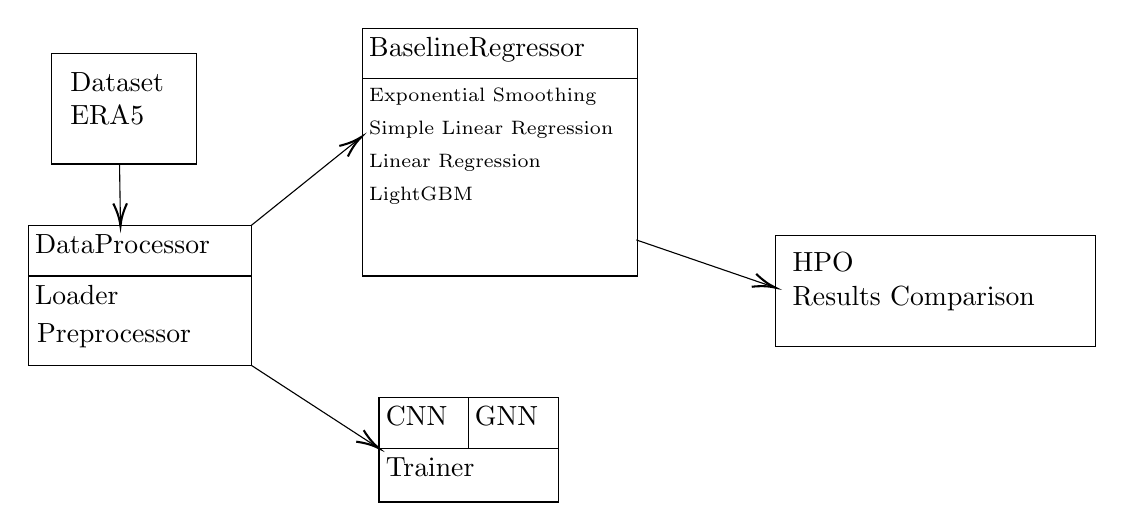
\begin{tikzpicture}[x=0.75pt,y=0.75pt,yscale=-1,xscale=1]
\draw   (49,24) -- (119,24) -- (119,77.4) -- (49,77.4) -- cycle ;
\draw   (38,107) -- (145.47,107) -- (145.47,131.4) -- (38,131.4) -- cycle ;
\draw   (199,12) -- (331.47,12) -- (331.47,36.4) -- (199,36.4) -- cycle ;
\draw   (38,131.4) -- (145.47,131.4) -- (145.47,174.4) -- (38,174.4) -- cycle ;
\draw   (199,36.4) -- (331.47,36.4) -- (331.47,131.4) -- (199,131.4) -- cycle ;
\draw    (82,78) -- (82.42,105.35) ;
\draw [shift={(82.45,107.35)}, rotate = 269.12] [color={rgb, 255:red, 0; green, 0; blue, 0 }  ][line width=0.75]    (10.93,-3.29) .. controls (6.95,-1.4) and (3.31,-0.3) .. (0,0) .. controls (3.31,0.3) and (6.95,1.4) .. (10.93,3.29)   ;
\draw    (145.47,107) -- (196.91,65.65) ;
\draw [shift={(198.47,64.4)}, rotate = 141.21] [color={rgb, 255:red, 0; green, 0; blue, 0 }  ][line width=0.75]    (10.93,-3.29) .. controls (6.95,-1.4) and (3.31,-0.3) .. (0,0) .. controls (3.31,0.3) and (6.95,1.4) .. (10.93,3.29)   ;
\draw   (207,190) -- (293.47,190) -- (293.47,214.4) -- (207,214.4) -- cycle ;
\draw   (207,214.4) -- (293.47,214.4) -- (293.47,240.27) -- (207,240.27) -- cycle ;
\draw    (250.1,190.17) -- (250.1,214.17) ;
\draw    (145.47,174.4) -- (205.32,213.31) ;
\draw [shift={(207,214.4)}, rotate = 213.03] [color={rgb, 255:red, 0; green, 0; blue, 0 }  ][line width=0.75]    (10.93,-3.29) .. controls (6.95,-1.4) and (3.31,-0.3) .. (0,0) .. controls (3.31,0.3) and (6.95,1.4) .. (10.93,3.29)   ;
\draw   (398,112) -- (552,112) -- (552,165.4) -- (398,165.4) -- cycle ;
\draw    (331,114) -- (396.11,136.35) ;
\draw [shift={(398,137)}, rotate = 198.95] [color={rgb, 255:red, 0; green, 0; blue, 0 }  ][line width=0.75]    (10.93,-3.29) .. controls (6.95,-1.4) and (3.31,-0.3) .. (0,0) .. controls (3.31,0.3) and (6.95,1.4) .. (10.93,3.29)   ;
\draw (57,32) node [anchor=north west][inner sep=0.75pt]   [align=left] {Dataset\\ERA5};
\draw (40,110) node [anchor=north west][inner sep=0.75pt]   [align=left] {DataProcessor};
\draw (40,134.4) node [anchor=north west][inner sep=0.75pt]   [align=left] {Loader};
\draw (41,153) node [anchor=north west][inner sep=0.75pt]   [align=left] {Preprocessor};
\draw (201,15) node [anchor=north west][inner sep=0.75pt]   [align=left] {BaselineRegressor};
\draw (201,39.4) node [anchor=north west][inner sep=0.75pt]   [align=left] {{\scriptsize Exponential Smoothing}\\{\scriptsize Simple Linear Regression}\\{\scriptsize Linear Regression}\\{\scriptsize LightGBM}};
\draw (209,193) node [anchor=north west][inner sep=0.75pt]   [align=left] {CNN \ \ GNN};
\draw (209,217.4) node [anchor=north west][inner sep=0.75pt]   [align=left] {Trainer};
\draw (405,119) node [anchor=north west][inner sep=0.75pt]   [align=left] {HPO \\Results Comparison};
\end{tikzpicture}
    \label{fig:proj-structure}
\end{figure}


\section{Dataset description}\label{chap:dataset}
Description of dataset, train, val, test split, resoution of data, generally all details.
\begin{itemize}
    \item Motivation behind usage of GRIB files and their description.
\end{itemize}

\section{Preprocessing methods}
Dividing time series into window sequences, normalization techniques

\section{Experiments}
We experimented with various solutions involving different numbers of layers and regularization techniques. Surprisingly, a relatively shallow network consistently outperformed all other solutions. As a result, there was no need to introduce any regularization techniques except LayerNorm, as overfitting was not observed.

\subsection{Hyperparameters optimization}
A short definition of Bayesian optimization and presentation of used Optuna sampler - Tree-Structured Parzen Estimator.~\cite{watanabe2023treestructured} 

\section{Results}
Results presentation, comparision with other models/benchmark scores. Visualisation and analysis.

\section{Practical details}
Explain training, evaluating and forecasting details and methods - e.g. spatial mapping of neural nets;
normalization and regularization techniques, used metrics and objectives, post processing, computation time, software and hardware stack etc. 

\chapter{Application}

\section{Functionality}
\section{API}
\section{Data Storage and DevOps solutions}

\chapter{Conclusions}
\section{Conclusions}
One of the main goals of the thesis was to introduce and compare the performance of several machine learning methods concerning the weather forecasting task and to prove the hypothesis that these methods are promising in the context of future research. We believe that we have succeeded in this goal, in fact, we were even surprised by the quality of some solutions. Unexpectedly, even very naive methods, such as ridge regression, return satisfactory results. Another goal that we successfully achieved was the implementation of a model based on graph neural networks, which, proved to be very light and leverage a small number of parameters, which was not a part of our initial objective. Its results definitely beat other methods and approached the overall performance of an arbitrarily chosen topline, while beating it on features related to pressure and precipitation. This is yet another indication that MLWP methods will be crucial in future approaches to the weather forecasting. Analyses of the quality of solutions depending on the length of the input sequence and the predicted one have confirmed our hypotheses, and recently we have even managed to improve the predictive performance of the topline using a linear combination of its predictions with those returned by our graph architecture.

Limitations associated with the top-performing model, are related to its dissatisfactory predictive capabilities in terms of forecasting on features with challenging distributions, i.e. total precipitation and cloud cover.

\section{Future perspectives}
Future enhancements may include refining the graph architecture structure by integrating additional components previously mentioned in the literature review section. An illustrative approach may be the incorporation of fine-tuning with the autoregressive objective function, similar as was the case for FourCastNet (Section \ref{sec:fourcastnet}). 


Reconstructing our entire training pipeline so that the autoregressive optimization process would be performed at every training step also seems reasonable and worth analyzing. 


Detailed research in the area related to transformer-based architectures is also encouraging, as a suggestion we propose the usage of Vision Transformer as presented in MetNet to enrich our spatial context. Another idea might be to incorporate the ability of recurrent neural networks or attention mechanism to build even better temporal representation. 


It also seems an interesting idea to perform further experiments in the context of creating hybrid models from the solutions we have already implemented -- one might be to combine models with low correlation to form ensembles and see how such a solution would perform. 

Retraining and evaluating implemented solutions, while excluding features with challenging distributions, also seems natural. An interesting experiment would be to remove hard-to-predict features, such as total cloud cover and total precipitation, from the dataset. Since forecasting these variables is difficult, omitting them might yield better results for predicting other features.

In addition, in the case of gaining access to sufficient computing resources, we would be eager to test our architecture and the entire framework for analyzing its behavior for data from a period of more than one year and also from larger boundaries than those covering the administrative area of Poland. It is worth noting that increased computational power would also enable the prediction of additional features and extreme weather conditions.

It would be worth comparing the quality of predictions based on the prediction hour, not just the month. Finally, we believe training and evaluating the models using a more granular interval between timestamps, for example every 1 or 2 hours, would be an interesting analysis.


% 
\chapter{Wstęp}

Wstęp do pracy powinien zawierać następujące elementy:
\begin{itemize}
    \item krótkie uzasadnienie podjęcia tematu; 
    \item cel pracy (patrz niżej); 
    \item zakres (przedmiotowy, podmiotowy, czasowy) wyjaśniający, w jakim rozmiarze praca będzie realizowana; 
    \item ewentualne hipotezy, które autor zamierza sprawdzić lub udowodnić; 
    \item krótką charakterystykę źródeł, zwłaszcza literaturowych; 
    \item układ pracy (patrz niżej), czyli zwięzłą charakterystykę zawartości poszczególnych rozdziałów; 
    \item ewentualne uwagi dotyczące realizacji tematu pracy np.~trudności, które pojawiły się w trakcie 
    realizacji poszczególnych zadań, uwagi dotyczące wykorzystywanego sprzętu, współpraca z firmami zewnętrznymi. 
\end{itemize}

\noindent
\textbf{Wstęp do pracy musi się kończyć dwoma następującymi akapitami:}
\begin{quote}
Celem pracy jest opracowanie / wykonanie analizy / zaprojektowanie / ...........
\end{quote}
oraz:
\begin{quote}
Struktura pracy jest następująca. W rozdziale 2 przedstawiono przegląd literatury na temat ........ 
Rozdział 3 jest poświęcony ....... (kilka zdań). 
Rozdział 4 zawiera ..... (kilka zdań) ............ itd. 
Rozdział X stanowi podsumowanie pracy. 
\end{quote}

W przypadku prac inżynierskich zespołowych lub magisterskich 2-osobowych, po tych dwóch w/w akapitach 
musi w pracy znaleźć się akapit, w którym będzie opisany udział w pracy poszczególnych członków zespołu. Na przykład:

\begin{quote}
Jan Kowalski w ramach niniejszej pracy wykonał projekt tego i tego, opracował ......
Grzegorz Brzęczyszczykiewicz wykonał ......, itd. 
\end{quote}


% 
\chapter{Podstawy teoretyczne}

Rozdział teoretyczny --- przegląd literatury naświetlający stan wiedzy na dany temat. 

Przegląd literatury naświetlający stan wiedzy na dany temat obejmuje rozdziały pisane na podstawie
literatury, której wykaz zamieszczany jest w części pracy pt.~\emph{Literatura} (lub inaczej \emph{Bibliografia},
\emph{Piśmiennictwo}). W tekście pracy muszą wystąpić odwołania do wszystkich pozycji zamieszczonych w
wykazie literatury. \textbf{Nie należy odnośników do literatury umieszczać w stopce strony.} Student jest
bezwzględnie zobowiązany do wskazywania źródeł pochodzenia informacji przedstawianych w pracy,
dotyczy to również rysunków, tabel, fragmentów kodu źródłowego programów itd. Należy także podać
adresy stron internetowych w przypadku źródeł pochodzących z Internetu.



% 
\chapter{Rozwinięcie}

Rozdziały dokumentujące pracę własną studenta: opisujące ideę, sposób lub metodę 
rozwiązania postawionego problemu oraz rozdziały opisujące techniczną stronę rozwiązania 
--- dokumentacja techniczna, przeprowadzone testy, badania i uzyskane wyniki. 

Praca musi zawierać elementy pracy własnej autora adekwatne do jego wiedzy praktycznej uzyskanej w
okresie studiów. Za pracę własną autora można uznać np.: stworzenie aplikacji informatycznej lub jej
fragmentu, zaproponowanie algorytmu rozwiązania problemu szczegółowego, przedstawienie projektu 
np.~systemu informatycznego lub sieci komputerowej, analizę i ocenę nowych technologii lub rozwiązań
informatycznych wykorzystywanych w przedsiębiorstwach, itp. 

Autor powinien zadbać o właściwą dokumentację pracy własnej obejmującą specyfikację założeń i 
sposób realizacji poszczególnych zadań
wraz z ich oceną i opisem napotkanych problemów. W przypadku prac o charakterze 
projektowo-implementacyjnym, ta część pracy jest zastępowana dokumentacją techniczną i użytkową systemu. 

W pracy \textbf{nie należy zamieszczać całego kodu źródłowego} opracowanych programów. Kod źródłowy napisanych
programów, wszelkie oprogramowanie wytworzone i wykorzystane w pracy, wyniki przeprowadzonych
eksperymentów powinny być umieszczone np. na płycie CD, stanowiącej dodatek do pracy.

\section*{Styl tekstu}

Należy\footnote{Uwagi o stylu pochodzą częściowo ze stron prof. Macieja Drozdowskiego~\cite{Drozdowski2006}.} 
stosować formę bezosobową, tj.~\emph{w pracy rozważono ......, 
w ramach pracy zaprojektowano ....}, a nie: \emph{w pracy rozważyłem, w ramach pracy zaprojektowałem}. 
Odwołania do wcześniejszych fragmentów tekstu powinny mieć następującą postać: ,,Jak wspomniano wcześniej, ....'', 
,,Jak wykazano powyżej ....''. Należy unikać długich zdań. 

Niedopuszczalne są zwroty używane w języku potocznym. W pracy należy używać terminologii informatycznej, która ma 
sprecyzowaną treść i znaczenie. 

Niedopuszczalne jest pisanie pracy metodą \emph{cut\&paste}, bo jest to plagiat i dowód intelektualnej indolencji autora.
Dane zagadnienie należy opisać własnymi słowami. Zawsze trzeba powołać się na zewnętrzne źródła. 


% 
\chapter{Zakończenie}

Zakończenie pracy zwane również Uwagami końcowymi lub Podsumowaniem powinno zawierać ustosunkowanie
się autora do zadań wskazanych we wstępie do pracy, a w szczególności do celu i zakresu pracy oraz
porównanie ich z faktycznymi wynikami pracy. Podejście takie umożliwia jasne określenie stopnia
realizacji założonych celów oraz zwrócenie uwagi na wyniki osiągnięte przez autora w ramach jego
samodzielnej pracy.

Integralną częścią pracy są również dodatki, aneksy i załączniki zawierające stworzone w ramach pracy programy, aplikacje i projekty.


%--------------------------------------
% Literatura
%--------------------------------------

\bibliographystyle{plain}{\raggedright\sloppy\small\bibliography{bibliografia}}

%--------------------------------------
% Dodatki
%--------------------------------------

\cleardoublepage
\appendix
\newpage

\chapter{Składanie dokumentu w systemie \LaTeX}

W tym rozdziale znajduje się
garść informacji o tym, jak poprawnie składać tekst pracy w systemie \LaTeX{} wraz z 
przykładami, które mają służyć do przeklejania do własnych dokumentów.

\section{Struktura dokumentu}
\chaptermark{Tytuł rozdziału, jeśli pełen się nie mieści\ldots{}}{}

Praca składa się z rozdziałów (\texttt{chapter}) i podrozdziałów (\texttt{section}).
Ewentualnie można również rozdziały zagnieżdzać (\texttt{subsection}, \texttt{subsubsection}),
jednak nie powinno się wykraczać poza drugi poziom hierarchii (czyli \texttt{subsubsection}).

\section{Akapity i znaki specjalne}

Akapity rozdziela się od siebie przynajmniej jedną pustą linią. Podstawowe
instrukcje, które się przydają to \emph{wyróżnienie pewnych słów}. Można również
stosować \textbf{styl pogrubiony}, choć nie jest to generalnie zalecane.

Należy pamiętać o zasadach polskiej interpunkcji i ortografii. Po spójnikach 
jednoliterowych warto wstawić znak tyldy ($\sim$), który jest tak zwaną
,,twardą spacją'' i powoduje, że wyrazy nią połączone nie będą rozdzielane
na dwie linie tekstu.

Polskie znaki interpunkcyjne różnią się nieco od angielskich: to jest ,,polski'', a to jest
``angielski''. W kodzie źródłowym tego tekstu będzie widać różnicę.

Proszę również zwrócić uwagę na znak myślnika, który może być pauzą ,,---'' lub
półpauzą: ,,--''. Należy stosować je konsekwentnie. Do łączenia wyrazów używamy
zwykłego ,,-'' (\emph{północno-wschodni}), do myślników --- pauzy lub półpauzy.
Inne zasady interpunkcji i typografii można znaleźć w słownikach.

\section{Wypunktowania}

Wypunktowanie z cyframi:
\begin{enumerate}
    \item to jest punkt,
    \item i to jest punkt,
    \item a to jest ostatni punkt.
\end{enumerate}

\noindent
Po wypunktowaniach czasem nie warto wstawiać wcięcia akapitowego. Wtedy przydatne jest
polecenie \texttt{noindent}. Wypunktowanie z kropkami (tzw.~\emph{bullet list}) wygląda tak:
\begin{itemize}
    \item to jest punkt,
    \item i to jest punkt,
    \item a to jest ostatni punkt.
\end{itemize}

\noindent
Wypunktowania opisowe właściwie niewiele się różnią:
\begin{description}
    \item[elementA] to jest opis,
    \item[elementB] i to jest opis,
    \item[elementC] a to jest ostatni opis.
\end{description}


\section{Polecenia pakietu \texttt{ppfcmthesis}}

Parę poleceń zostało zdefiniowanych aby uspójnić styl pracy. Są one przedstawione poniżej
(oczywiście nie trzeba się do nich stosować).

\paragraph{Makra zdefiniowane dla języka angielskiego.} Są nimi: \texttt{termdef} oraz \texttt{acronym}.
Przykłady poniżej obrazują ich przewidywane użycie w tekście.
\begin{center}\footnotesize%
\begin{tabular}{l >{\rightskip\fill}p{12cm}}
\toprule
źródło   & \texttt{we call this a $\backslash$termdef\{Database Management System\} ($\backslash$acronym\{DBMS\})} \\ \cmidrule(lr){2-2}
docelowo & we call this a \termdef{Database Management System} (\acronym{DBMS}) \\ 
\bottomrule
\end{tabular}
\end{center}

\paragraph{Makra zdefiniowane dla języka polskiego.} Podobnie jak dla języka angielskiego zdefiniowano
odpowiedniki polskie: \texttt{defini\-cja}, \texttt{akronim} oraz \texttt{english} dla tłumaczeń angielskich
terminów. Przykłady poniżej obrazują ich przewidywane użycie w tekście.
\begin{center}\footnotesize%
\begin{tabular}{l >{\rightskip\fill}p{12cm}}
\toprule
źródło   & \texttt{nazywamy go $\backslash$definicja\{systemem zarządzania bazą danych\} ($\backslash$akronim\{DBMS\}, $\backslash$english\{Database Management System\})} \\ \cmidrule(lr){2-2}
docelowo & nazywamy go \definicja{systemem zarządzania bazą danych} (\akronim{DBMS}, \english{Database Management System}) \\ \bottomrule
\end{tabular}
\end{center}


\section{Rysunki}

Wszystkie rysunki (w tym również diagramy, szkice i inne) osadzamy w środowisku 
\texttt{figure} i umieszczamy podpis \emph{pod} rysunkiem, w formie elementu \texttt{caption}. Rysunki powinny
zostać umieszczone u góry strony (osadzone bezpośrednio w treści strony zwykle utrudniają czytanie tekstu).
Rysunek~\ref{rys:plama} zawiera przykład pełnego osadzenia rysunku na stronie.

\begin{figure}[t] % możliwe opcje to 't' - top, 'b' - bottom, 'h' - 'here', ale zaleca się 't'
\centering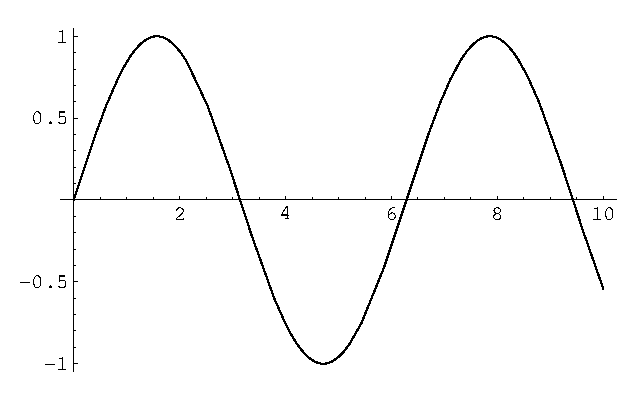
\includegraphics[width=5cm]{figures/mathematica}
\caption{Wykres.}\label{rys:plama}
\end{figure}

\begin{figure}[t]
\centering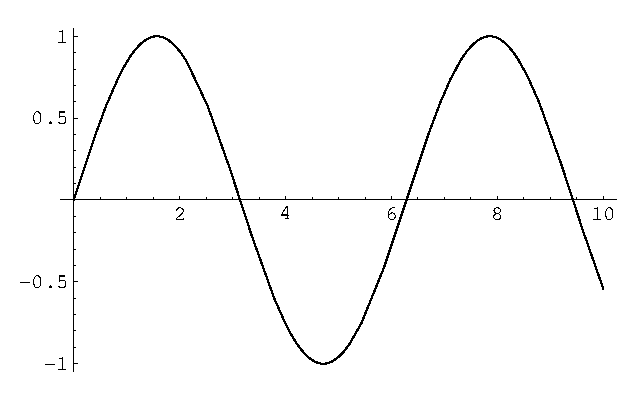
\includegraphics[width=\textwidth]{figures/mathematica}
\fcmfcaption{Ten sam wykres ale na szerokość tekstu. Formatowanie podpisu zgodne z wytycznymi FCMu.}\label{rys:plama2}
\end{figure}

Styl FCMu to nieco inne nagłówki rysunków. Dostepne są one poleceniem \texttt{fcmfcaption} (zob.~rysunek
\ref{rys:plama2}).

\subsection{Tablice}

Tablice to piękna rzecz, choć akurat ich umiejętne tworzenie w \LaTeX{}u nie jest łatwe. 
Jeśli tablica jest skomplikowana, to można ją na przykład wykonać w programie
OpenOffice, a następnie wyeksportować jako plik \akronim{PDF}. W każdym przypadku tablice wstawia się podobnie
jak rysunki, tylko że w środowisko \texttt{table}. Tradycja typograficzna sugeruje umieszczenie opisu tablicy, a więc
elementu \texttt{caption} ponad jej treścią (inaczej niż przy rysunkach).  

Tablica~\ref{tab:tabela} pokazuje pełen przykład.

\begin{table}[ht]
\caption{Przykładowa tabela. Styl opisu jest zgodny z rysunkami.}\label{tab:tabela}
\centering\footnotesize%
\begin{tabular}{l c}
\toprule
artykuł & cena [zł] \\
\midrule
bułka   & $0,4$ \\
masło   & $2,5$ \\
\bottomrule
\end{tabular}
\end{table}

Zasady FCMu sugerują nieco inne nagłówki tablic. Dostepne są one poleceniem \texttt{fcmtcaption} (zob.~tablicę
\ref{tab:tabela2}).

\begin{table}[ht]
\fcmtcaption{Przykładowa tabela. Styl opisu jest zgodny z wytycznymi FCMu.}\label{tab:tabela2}
\centering\footnotesize%
\begin{tabular}{l c}
\toprule
artykuł & cena [zł] \\
\midrule
bułka   & $0,4$ \\
masło   & $2,5$ \\
\bottomrule
\end{tabular}
\end{table}


\subsection{Checklista}

\begin{itemize}
\item Znakiem myślnika jest w LaTeXu dywiz pełen (---) albo półpauza (--), przykład:
  A niech to jasna cholera --- wrzasnąłem.

\item Połączenie między wyrazami to zwykły myślnik, przykład:   północno-zachodni

\item Sprawdź czy tutuł pracy ma maksymalnie dwa wiersze i czy stanowią one pełne frazy
  (czy nie ma przeniesienia bez sensu).

\item Sprawdź ostrzeżenia o 'overfull' i 'underful' boxes. Niektóre z nich można zignorować (spójrz
  na wynik formatowania), niektóre trzeba poprawić; czasem przeformułować zdanie.

item Przypisy stawia się wewnątrz zdań lub za kropką, przykład:
  Footnote is added after a comma.\footnote{Here is a footnote.}

\item Nie używaj przypisów zbyt często. Zobacz, czy nie lepiej będzie zintegrować przypis z tekstem.

\item Tytuły tabel, rysunków powinny kończyć się kropką.

\item Nie używaj modyfikatora [h] (here) do rysunków i tabel. Rysunki i tabele powinny być
  justowane do góry strony lub na stronie osobnej.

\item Wyróżnienie w tekście to polecenie \emph{wyraz}, nie należy używać czcionki pogrubionej (która
  wystaje wizualnie z tekstu i rozprasza).

\item Nazwy plików, katalogów, ścieżek, zmiennych środowiskowych, klas i metod formatujemy poleceniem
  \texttt{plik\_o\_pewnej\_nazwie}.

\item Po ostatniej zmianie do treści, sprawdź i przenieś wiszące spójniki wstawiając przed nie znak
  tyldy (twardej spacji), przykład:
  Ala i~kotek nie lubią mleczka, a~Stasiu lubi.
  
\item Za i.e. (id est) i e.g. (exempli gratia) stawia się zwyczajowo przecinek w typografii amerykańskiej.

\item Przed i za pełną pauza nie ma zwyczajowo spacji w typografii amerykańskiej, przykład:
  Darn, this looks good---said Mary.

\item Zamykający cudzysłów oraz footnote wychodzą za ostatni znak interpunkcji w typografii 
  amerykańskiej, przykłady:
  It can be called a ``curiosity,'' but it's actually normal.
  Footnote is added after a comma.\footnote{Here is a footnote.}

\item Odwołania do tabel i rysunków zawsze z wielkiej litery, przykład:
  In Figure~\ref{rys:plama} we illustrated XXX and in Table~\ref{tab:tabela} we show detailed data.
  
\end{itemize}


\section{Literatura i materiały dodatkowe}

Materiałów jest mnóstwo. Oto parę z nich:
\begin{itemize}
    \item \emph{The Not So Short Introduction\ldots}, która posiada również tłumaczenie 
    w języku polskim.\\
    \url{http://www.ctan.org/tex-archive/info/lshort/english/lshort.pdf}

    \item Klasy stylu \texttt{memoir} posiadają bardzo wiele informacji o składzie tekstów
    anglosaskich oraz sposoby dostosowania \LaTeX{}a do własnych potrzeb.\\
    \url{http://www.ctan.org/tex-archive/macros/latex/contrib/memoir/memman.pdf}
    
    \item Nasza grupa dyskusyjna i repozytorium Git są również dobrym miejscem aby zapytać
    (lub sprawdzić czy pytanie nie zostało już zadane).\\
    \url{https://github.com/politechnika/put-latex}

    \item Dla łaknących więcej wiedzy o systemie LaTeX podstawowym źródłem informacji
    jest książka Lamporta~\cite{Lamport1985}. Prawdziwy \emph{hardcore} to oczywiście
    \emph{The \TeX{}book} profesora Knutha~\cite{Knuth1986}.
\end{itemize}



%--------------------------------------
% Informacja o prawach autorskich
%--------------------------------------

\ppcolophon

\end{document}
